\documentclass[onlymath,xcolor=pdftex,dvipsnames,table]{beamer}
\usefonttheme{serif}

\usepackage{array}
\usepackage{color}
\usepackage{xspace}
\usepackage{graphicx}
\usepackage{subfigure}
\usepackage{pstricks}
\usepackage{booktabs}
\usepackage{listings}
\usepackage{multimedia}
%\usepackage{beamerthemeshadow}
\usepackage{amsmath,amsfonts,amsthm,amssymb}
\usepackage[noend]{algpseudocode}
\usepackage{algorithm}
\usepackage{algorithmicx}
\usepackage{transparent} % transparent background
\usepackage{etoolbox}

\usetheme{Singapore}
%\usefonttheme{serif}
%\useoutertheme{infolines}
%\setbeamertemplate{background canvas}[vertical shading]
%				     [bottom=red!10,top=blue!10]

%---------- header setting ------------------------------------------------%
% a flag that tells us how the circles should be drawn
\newif\ifnavbeforecurrent
% reset the flag before every navigation bar
\pretocmd\insertnavigation{\navbeforecurrenttrue}{}{}

% change the circle drawing code so that it changes based on the flag
\defbeamertemplate*{mini frame in current subsection}{changing}[1][50]
{%
  \begin{pgfpicture}{0pt}{0pt}{0.1cm}{0.1cm}
    \pgfpathcircle{\pgfpoint{0.05cm}{0.05cm}}{0.05cm}
    \ifnavbeforecurrent
        \pgfusepath{fill,stroke}
    \else
        \pgfusepath{stroke}
    \fi
  \end{pgfpicture}%
}
\setbeamertemplate{mini frame in current subsection}[changing]

% after the circle for the current frame is drawn, change the flag
\defbeamertemplate*{mini frame}{changing}
{%
  \begin{pgfpicture}{0pt}{0pt}{0.1cm}{0.1cm}
    \pgfpathcircle{\pgfpoint{0.05cm}{0.05cm}}{0.05cm}
    \pgfusepath{fill,stroke}
  \end{pgfpicture}%
  \global\navbeforecurrentfalse
}
\setbeamertemplate{mini frame}[changing]

%---------- footer setting ------------------------------------------------%
\makeatletter
\setbeamertemplate{footline}
{
  \leavevmode%
  \hbox{%
  %\begin{beamercolorbox}[wd=.333333\paperwidth,ht=2.25ex,dp=2ex,center]{author in head/foot}%
  %  \usebeamerfont{author in head/foot}%
  %\insertshortauthor\hspace{1em}\beamer@ifempty{\insertshortinstitute}{}{(\insertshortinstitute)}
  %\end{beamercolorbox}%
  \begin{beamercolorbox}[wd=.5\paperwidth,ht=2.25ex,dp=2ex,left]{title in head/foot}%
    \usebeamerfont{title in head/foot}\hspace{1em}\insertshorttitle
  \end{beamercolorbox}%
  \begin{beamercolorbox}[wd=.5\paperwidth,ht=2.25ex,dp=2ex,right]{date in head/foot}%
    \usebeamerfont{date in head/foot}\insertshortdate{}\hspace*{2em}
    \insertframenumber{}/\inserttotalframenumber\hspace*{2ex} 
  \end{beamercolorbox}}%
  \vskip0pt%
}
\makeatother
% no navigation bar
\beamertemplatenavigationsymbolsempty
% only page number version below
%\setbeamertemplate{footline}[page number]

%---------- footnote setting ------------------------------------------------
\addtobeamertemplate{footnote}{\vspace{-6pt}\advance\hsize-0.5cm}{\vspace{6pt}}
\makeatletter
% Alternative A: footnote rule
\renewcommand*{\footnoterule}{\kern -3pt \hrule \@width 2in \kern 8.6pt}
% Alternative B: no footnote rule
% \renewcommand*{\footnoterule}{\kern 6pt}
\makeatother

{\setbeamertemplate{background canvas}{%
  %\begin{picture}(0,0)
  %  \put(302,-240){
  %    \includegraphics[width=0.15\paperwidth]{owl.jpg}}
  %\end{picture}}
\frame{\titlepage}}}

%---------- User-defined commands -----------------------------------------%
\newcommand{\probkb}{\textsc{ProbKB}\xspace}
\newcommand{\sherlock}{\textsc{Sherlock}\xspace}
\newcommand{\holmes}{\textsc{Holmes}\xspace}
\newcommand{\reverb}{\textsc{ReVerb}\xspace}
\newcommand{\tuffy}{\textsc{Tuffy}\xspace}
\newcommand{\felix}{\textsc{Felix}\xspace}
\newcommand{\alchemy}{\textsc{Alchemy}\xspace}
\newcommand{\blog}{\textsc{Blog}\xspace}
\newcommand{\nell}{\textsc{Nell}\xspace}
\newcommand{\probase}{\textsc{ProBase}\xspace}
\newcommand{\textrunner}{\textsc{TextRunner}\xspace}
\newcommand{\madden}{\textsc{MADden}\xspace}
\newcommand{\gist}{\textsc{GIST}\xspace}

\definecolor{darkblue}{rgb}{0,0,0.6}
\definecolor{darkred}{rgb}{0.6,0,0}

\let\oldemph\emph
\renewcommand{\emph}[1]{{\color{Blue}\oldemph{#1}}}
\newcommand{\define}[1]{\textit{#1}\xspace}
\newcommand{\strong}[1]{\textbf{#1}\xspace}
\newcommand{\stt}[1]{\texttt{\small #1}\xspace}

\newcommand{\head}[1]{{\large\color{OliveGreen}#1\\[2pt]}}


% declaration of the new block
\algblock{ParFor}{EndParFor}
% customising the new block
\algnewcommand\algorithmicparfor{\textbf{for}}
\algnewcommand\algorithmicpardo{\textbf{do in parallel}}
\algnewcommand\algorithmicendparfor{\textbf{barrier end}}
\algrenewtext{ParFor}[1]{\algorithmicparfor\ #1\ \algorithmicpardo}
\algrenewtext{EndParFor}{\algorithmicendparfor}

\definecolor{lightgray}{rgb}{0.98,0.98,0.98}
\hypersetup{colorlinks,linkcolor=,urlcolor=Blue}

\renewcommand{\ttdefault}{pcr}
\lstset{
  language=SQL,
  basicstyle={\footnotesize\ttfamily},
  numbers=none,
  backgroundcolor=\color{lightgray},
  aboveskip=3mm,
  belowskip=3mm,
  showstringspaces=false,
  columns=flexible,
  keywordstyle={\bfseries\color{Blue}},
  commentstyle={\color{Red}\textit},
  stringstyle=\color{Magenta},
  frame=single,
  breaklines=true,
  breakatwhitespace=true,
  tabsize=4
}

\AtBeginSubsection[]
{
 \begin{frame}
   \frametitle{Outline}
   \tableofcontents[currentsection,currentsubsection]
 \end{frame}
}

%% \AtBeginSection[]
%% {
%%   \begin{frame}
%%     \frametitle{Outline}
%%     \tableofcontents[currentsection,currentsubsection]
%%   \end{frame}
%% }

%\newlength{\wideitemsep}
%\setlength{\wideitemsep}{\itemsep}
%\addtolength{\wideitemsep}{5pt}
%\let\olditem\item
%\renewcommand{\item}{\setlength{\itemsep}{\wideitemsep}\olditem}

\title[\probkb Web-Scale Probabilistic Knowledge Base]%(optional, only for long titles)
{\probkb Web-Scale\\Probabilistic Knowledge Base}
\author % (optional, for multiple authors)
{Yang~Chen\\{\footnotesize\url{yang@cise.ufl.edu}}}
\institute[University of Florida] % (optional)
{
  Computer and Information Science and Engineering\\
  University of Florida\\
}
\date{Feb 22, 2012} % (optional)
\logo{
\includegraphics[width=3cm]{logo.pdf}}

\begin{document}

\maketitle

%---------- slide --------------------------------------------------%
\section{Introduction}
\subsection{Introduction}
\begin{frame}{Knowledge bases--Introduction}
\begin{itemize}
  \item A \emph{knowledge base}~\cite{nath2010efficient} is a special kind of database for knowledge management.
A knowledge base provides a means for information to be collected, organized,
shared, searched and utilized.
  \item A knowledge base helps machines understand humans, languages, and the world.
\end{itemize}
\begin{figure}
  \centering
  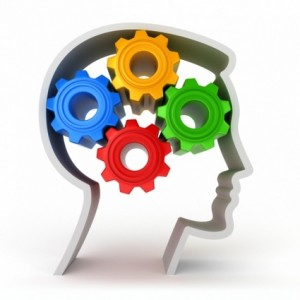
\includegraphics[width=.3\textwidth]{knowledgeBase.jpg}
\end{figure}
\end{frame}


%---------- slide --------------------------------------------------%
%% \begin{frame}{Knowledge bases--Introduction}
%% \begin{columns}[c]
%%   \column{0.46\textwidth}
%%   \begin{figure}
%%     \centering
%%     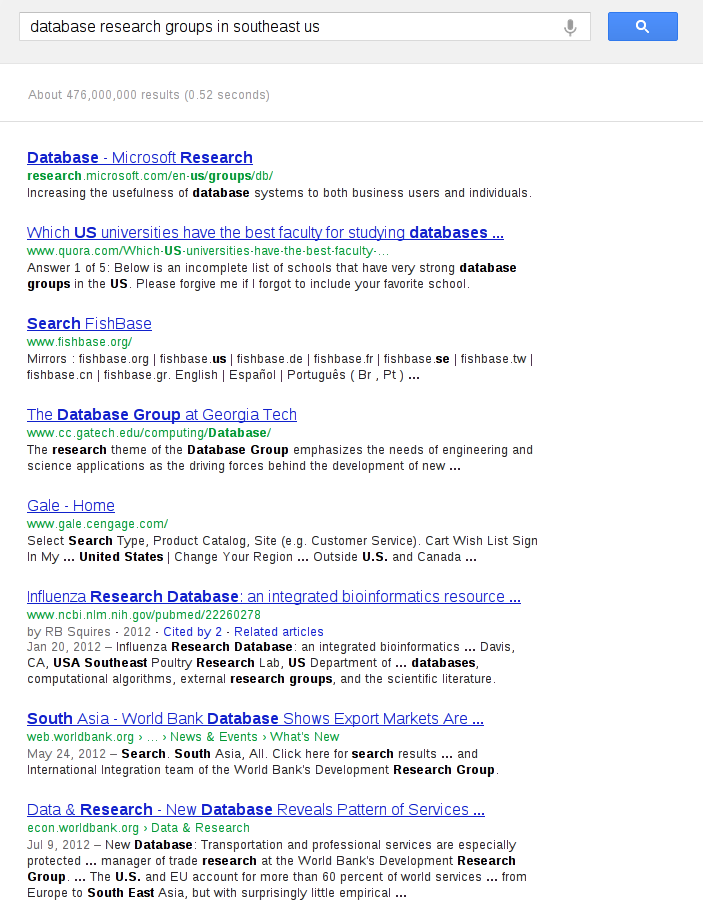
\includegraphics[width=\linewidth]{eg1.png}
%%   \end{figure}
%%   \column{0.46\textwidth}
%%   \begin{figure}
%%     \centering
%%     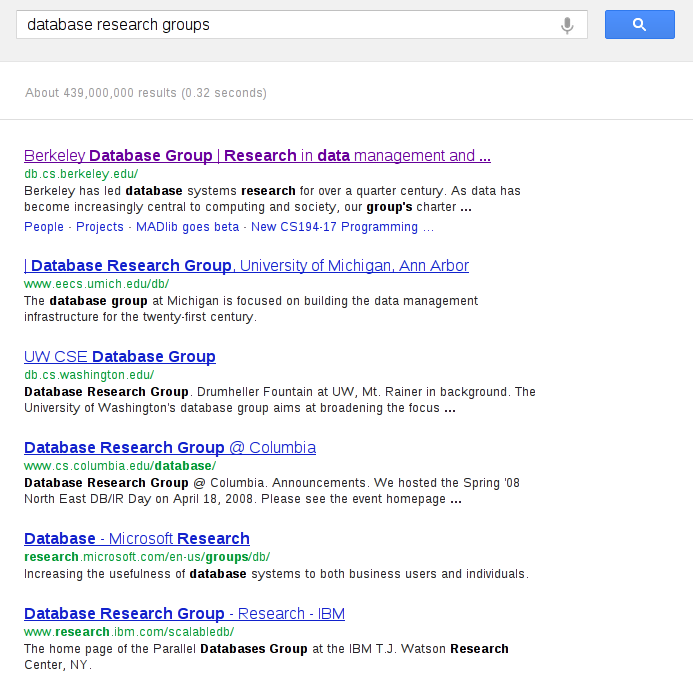
\includegraphics[width=\linewidth]{eg2.png}\\
%%     \line(1,0){150}\\
%%     
\includegraphics[width=\linewidth]{eg3.png}
%%   \end{figure}
%% \end{columns}
%% \end{frame}


%---------- slide --------------------------------------------------%
\subsection{Examples}
\begin{frame}{Examples}
\head{Google Knowledge Graph~\cite{googleknowledgegraph}}
\begin{columns}[c]
  \column{0.48\textwidth}
  \begin{figure}
    \centering
    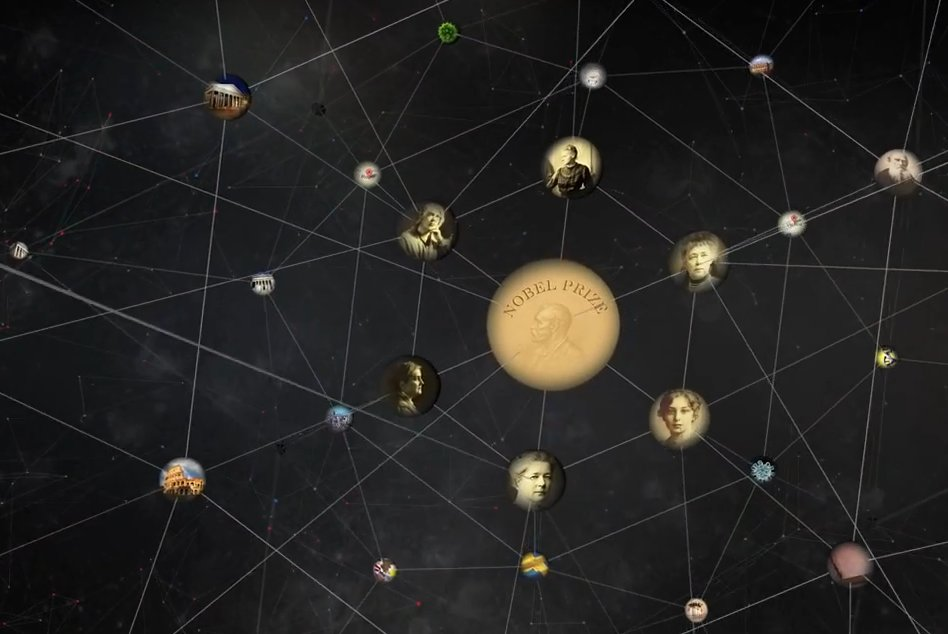
\includegraphics[width=\linewidth]{120701_google_knowledge_graph.jpg}
  \end{figure}
  \column{0.48\textwidth}
  \begin{figure}
    \centering
    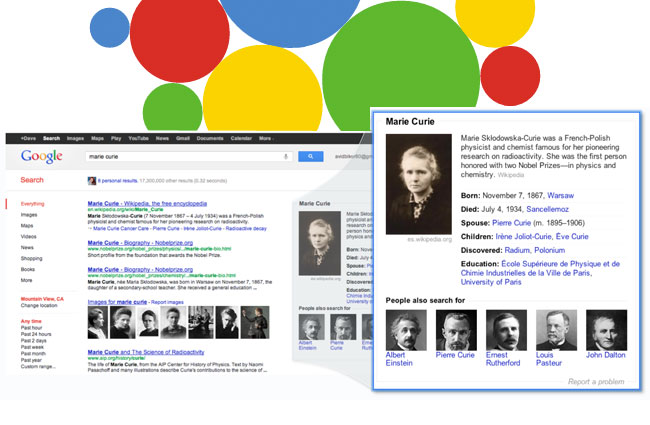
\includegraphics[width=\linewidth]{Google-Knowledge-Graph.jpg}
  \end{figure}
\end{columns}
\begin{center}
  \href{http://www.google.com/insidesearch/features/search/knowledge.html}{\large Demo}
\end{center}
\end{frame}


%---------- slide --------------------------------------------------%
%% \begin{frame}{Examples}
%% \head{\nell}
%% \nell~\cite{carlson2010toward} is a research project that attempts to create a computer system that learns over time to read the web.
%% \begin{figure}
%%   \centering
%%   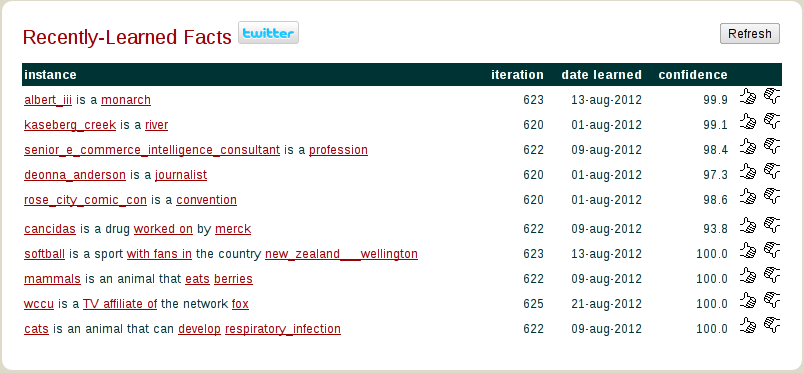
\includegraphics[width=.6\textwidth]{nell.png}
%% \end{figure}
%% Note that \nell produces uncertain results. This is typical among automatic extraction systems and is our major motivation to develop a large-scale probabilistic knowledge base.
%% \end{frame}


%---------- slide --------------------------------------------------%
\begin{frame}{Related Work}
\head{\sherlock-\holmes}
\begin{columns}[c]
  \column{0.45\textwidth}
  The \sherlock-\holmes~\cite{schoenmackers2011inference} is an open information extraction system consisting of two components:
  \begin{itemize}
    \item \sherlock~\cite{schoenmackers2010learning}, which learns inference rules offline, and
    \item \holmes~\cite{schoenmackers2008scaling}, which uses inference rules to answer queries online.
  \end{itemize}

  \column{0.45\textwidth}
  \begin{figure}
    \centering
    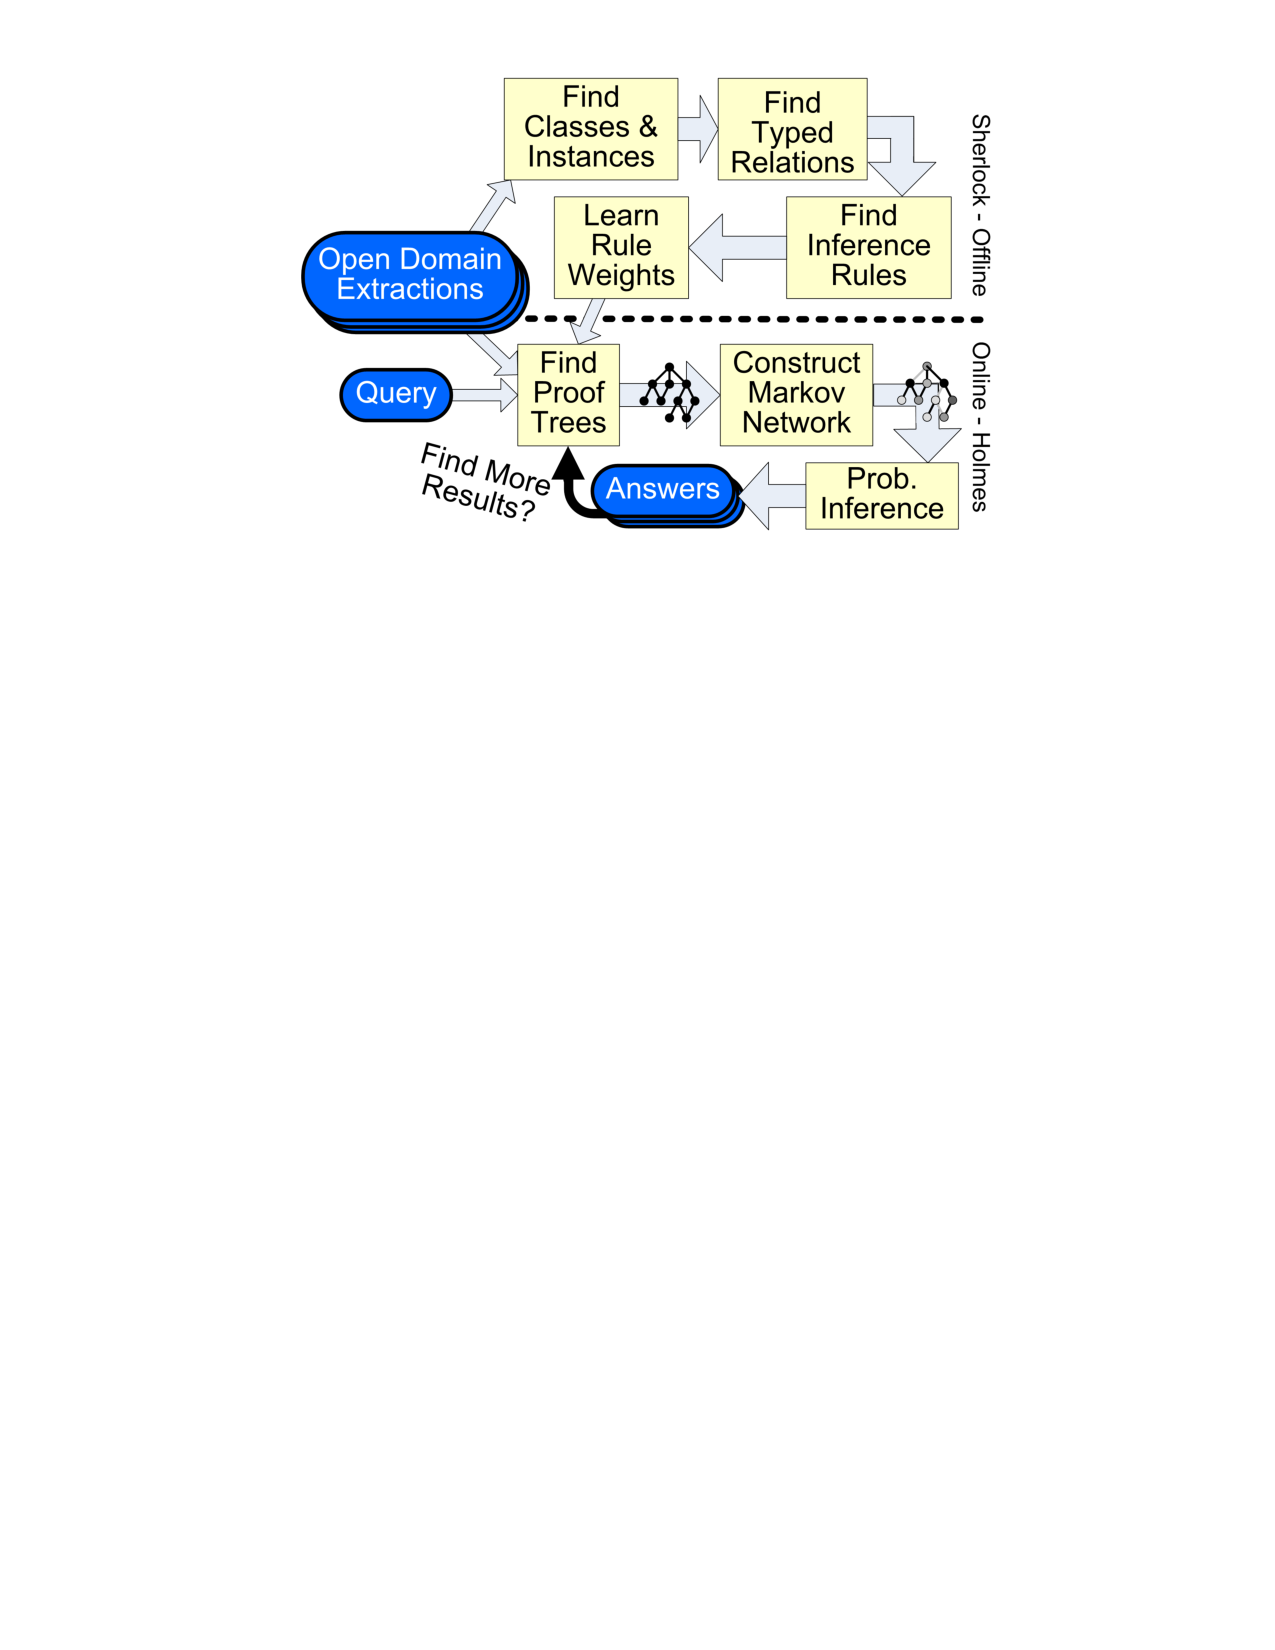
\includegraphics[clip,trim=125pt 500pt 125pt 30pt,width=\linewidth]{sherlock.pdf}
  \end{figure}
\end{columns}
\end{frame}


%---------- slide --------------------------------------------------%
\begin{frame}{Related Work}
\head{\tuffy-\felix}
The \tuffy-\felix~\cite{DBLP:journals/pvldb/NiuRDS11,2011arXiv1108.0294N} system is an Markov logic network~\cite{richardson2006markov} implementation that does large-scale probabilistic inference using an RDBMS.
\begin{columns}[c]
  \column{0.6\textwidth}
  \begin{itemize}
    \item A bottom-up approach to grounding using an RDBMS.
    \item A hybrid in-database grounding and in-memory inference architecture.
    \item Novel partitioning, loading, and parallel algorithms.
    \item Task decomposition to achieve web-scale.
  \end{itemize}

  \column{0.35\textwidth}
  \begin{figure}
    \centering
    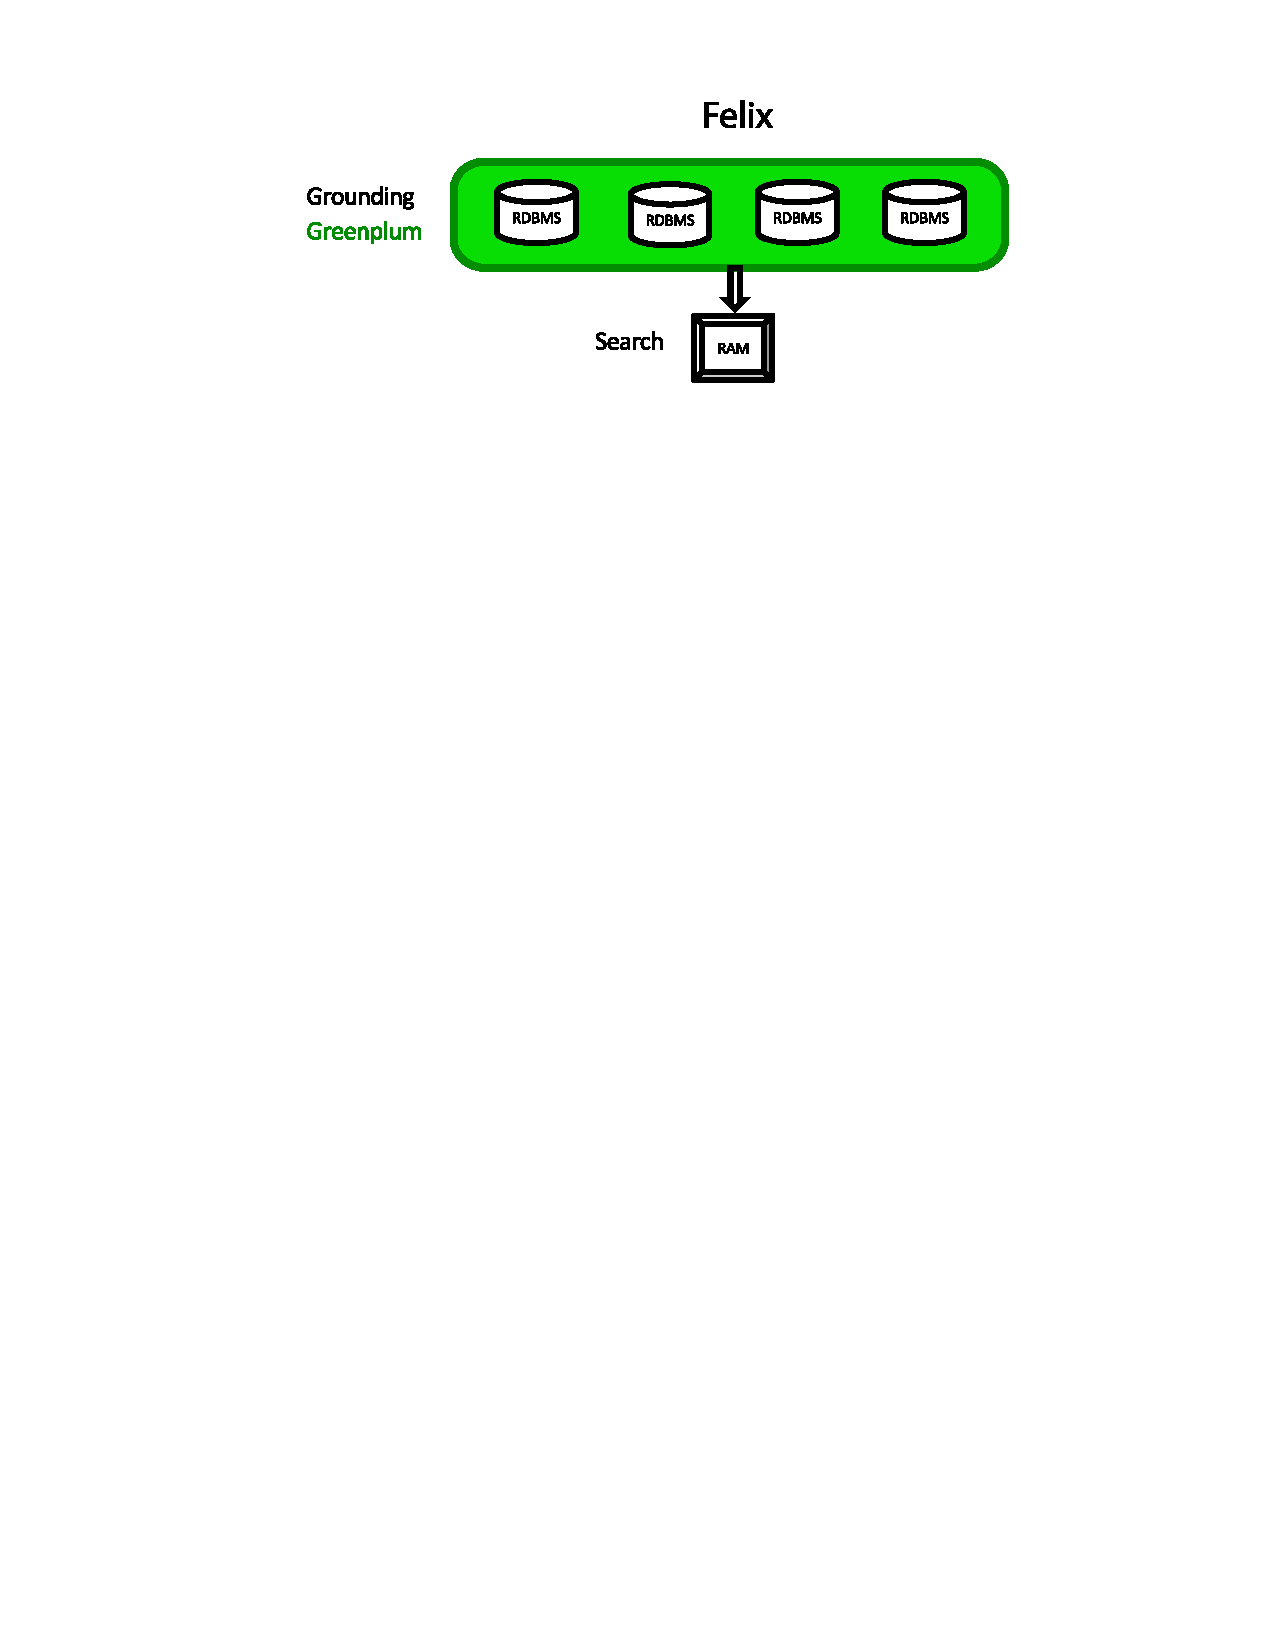
\includegraphics[clip,trim=125pt 500pt 125pt 30pt,width=\linewidth]{distfelix.pdf}
  \end{figure}
\end{columns}
\end{frame}


%---------- slide --------------------------------------------------%
\section{The \probkb System}
\subsection{\probkb Architecture}
\begin{frame}{Architecture}
\begin{figure}
  \centering
  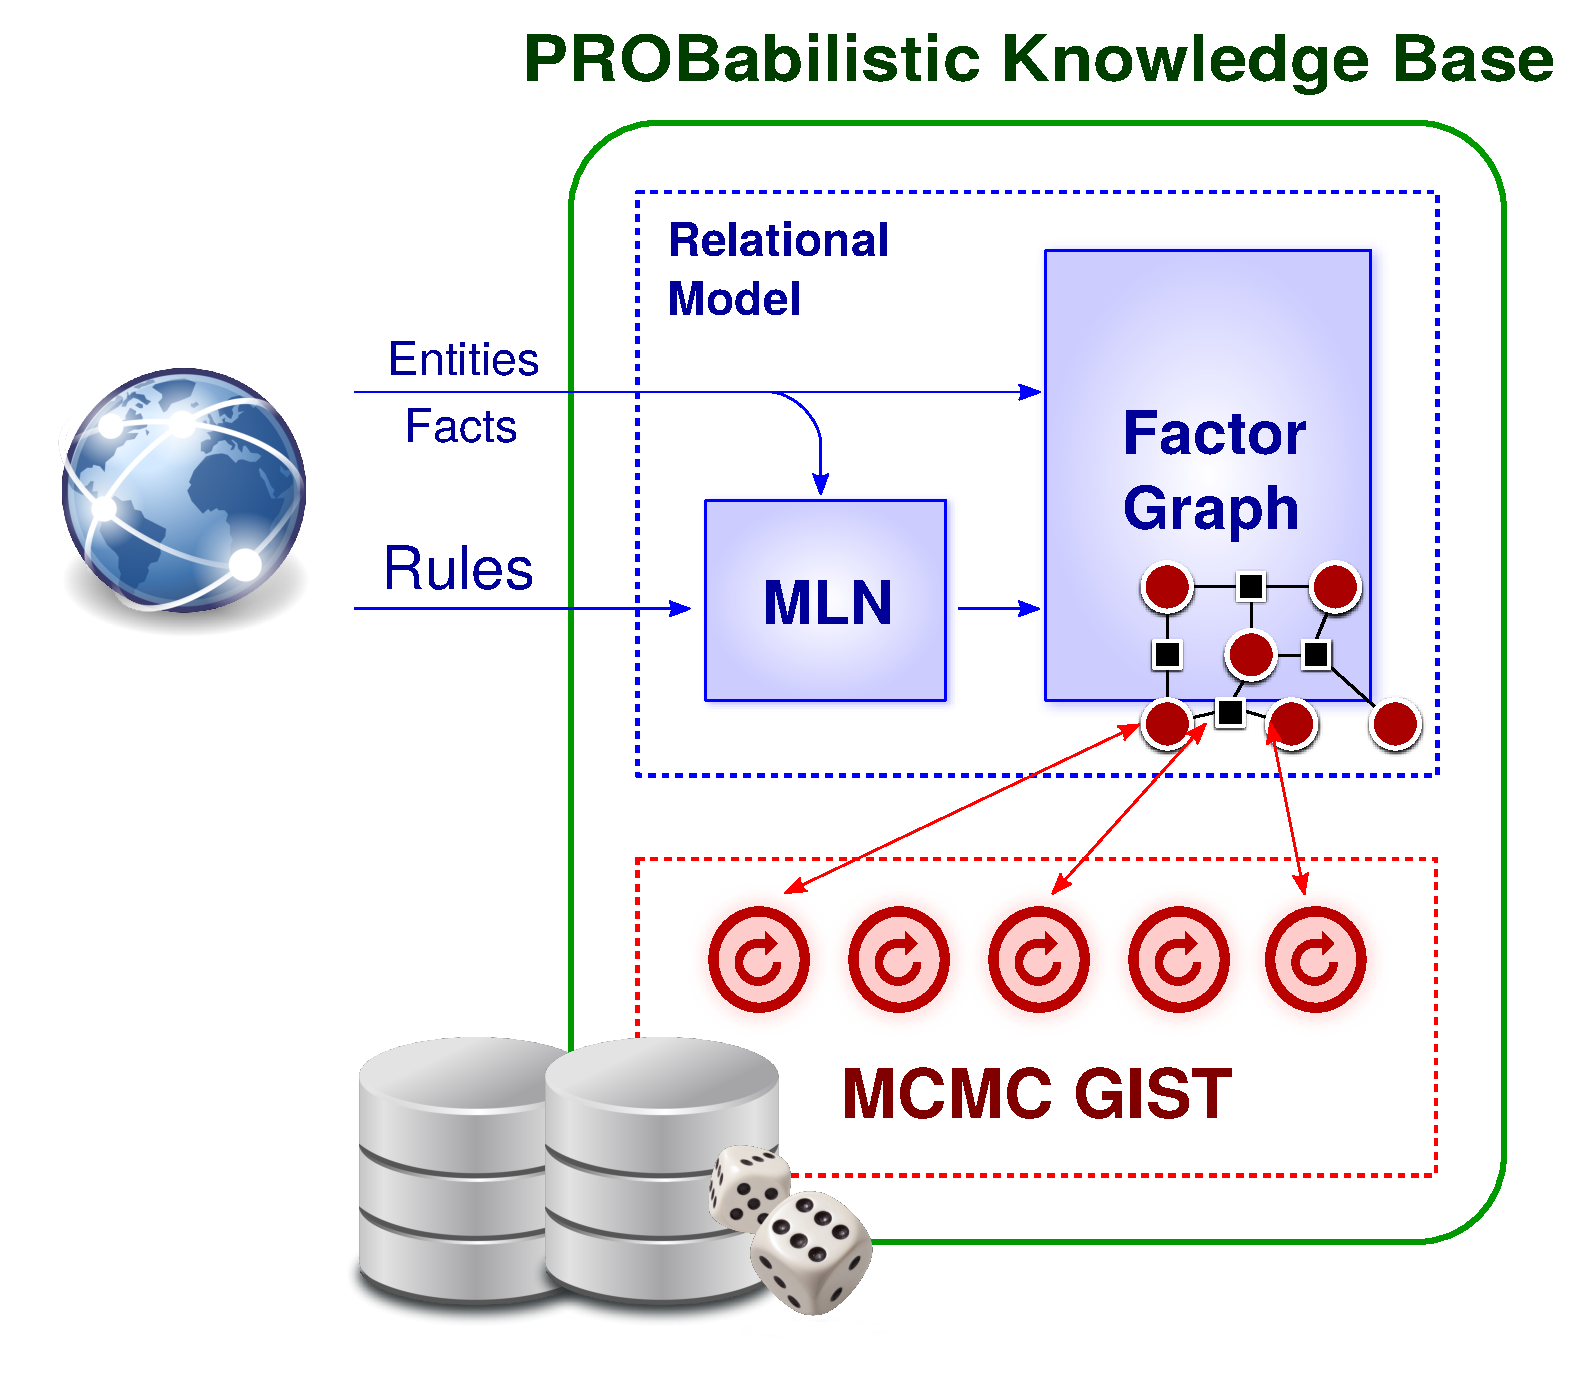
\includegraphics[clip,trim=30 0 15 0,width=.7\textwidth]{probkbarch.pdf}
\end{figure}
\end{frame}

%---------- slide --------------------------------------------------%
\begin{frame}{Architecture}
\head{Contributions}
\begin{itemize}
  \item A relation model for extracted entities, facts, and rules.
  \item Efficient grounding via at most a few relational operators.
  \item Parallel MCMC inference implemented as \stt{GIST} operations.
  \item Incremental inference: saving computation by focusing on least convergent variables.
\end{itemize}
\end{frame}

%---------- slide --------------------------------------------------%
\subsection{Markov Logic}
\begin{frame}{Markov Logic--Probabilistic Inference Framework}
A \emph{Markov logic network} (MLN)~\cite{richardson2006markov} is a set of formulae with weights. Together with a finite set of constants $C=\{c_1,\ldots,c_{\left\vert C\right\vert}\}$, it defines a Markov network.

\begin{columns}[c]
  \column{0.48\textwidth}
  \begin{table}\tiny
    \centering
    \begin{tabular}{cc}\toprule
      \textbf{Weight} & \textbf{First-Order Logic}\\\midrule
      0.7 & Fr($x$,$y$)$\wedge$Fr($y$,$z$)$\rightarrow$Fr($x$,$z$)\\
      1.5 & Sm($x$)$\rightarrow$Ca($x$)\\
      1.1 & Fr($x$,$y$)$\wedge$Sm($x$)$\rightarrow$Sm($y$)\\
      \bottomrule
    \end{tabular}
    \caption{Example Markov logic network.}
    \label{tab:mln}
  \end{table}

  \column{0.48\textwidth}
  A set of constants (entities, or objects) $$C=\{A,B\}.$$
\end{columns}\vspace{-25pt}
\begin{figure}
  \centering
  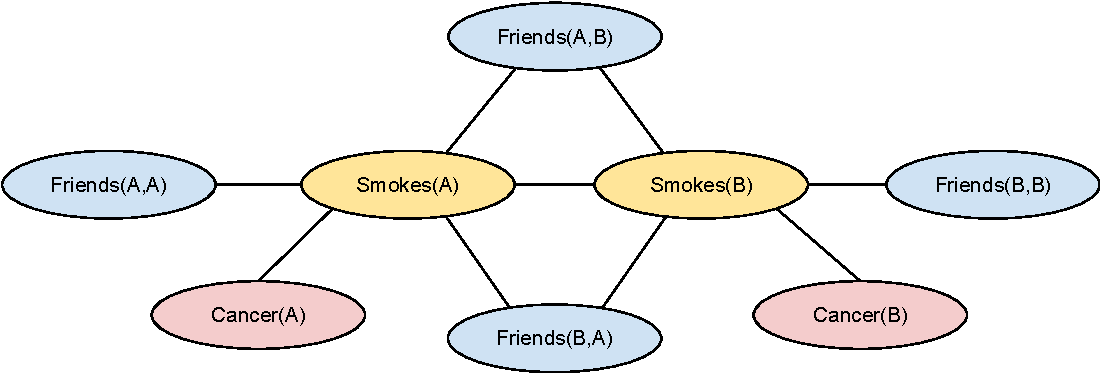
\includegraphics[clip,trim=40 35 40 40,width=0.75\textwidth]{mrf.pdf}
  \caption{Grounded Markov network.}
  \label{fig:ground}
\end{figure}
\end{frame}


%---------- slide --------------------------------------------------%
\begin{frame}{Grounding}
\emph{Grounding} is the process of substituting constants into MLN clauses.\\[5pt]

The result of grounding is a \emph{factor graph} (or \emph{Markov network}) from which we can infer marginal probabilities for individual facts.\\[15pt]

\head{Key Challenges}
\begin{itemize}
  \item Time-consuming, especially if the numbers of rules and entites are large.
  \item Grounded network has an intractably large size, making inference tasks slow.
\end{itemize}
\end{frame}


%---------- slide --------------------------------------------------%
\begin{frame}{Grounding}
\head{Scaling to the Web}
\begin{itemize}
  \item First-order Horn clauses:
  \begin{itemize}
    \item Avoids the need to enumerate ground atoms.
    \item Stored as \emph{first-class} citizen in RDBMS, grounding expressed as a few \stt{Join}s.
    \item Easier to learn than general first-order clauses.
  \end{itemize}
  \item Leveraging RDBMS query optimization techniques and possibly MPP frameworks (e.g. Greenplum).
  \item Ontology (typing): reducing the number of possible groundings and improving accuracy.
\end{itemize}
\end{frame}

%---------- slide --------------------------------------------------%
\begin{frame}[fragile]{Grounding}
A single \stt{JOIN} operation handles all rules of type
$$
p(x: c_1, y: c_2)\leftarrow q(x: c_1, z: c_3), r(z: c_3, y: c_2)
$$
\lstset{
  language=SQL,
  morekeywords=[2]{mln,relations,instances},
  keywordstyle=[2]{\color{OliveGreen}},
}
\begin{lstlisting}
SELECT DISTINCT mln.head AS head, mln.body1 AS body1, mln.body2 AS body2, r1.ent1 AS ent1, r1.ent2 AS ent2, r2.ent2 AS ent3
FROM relations r1, mln, relations r2, relations r3, instances i1, instances i2, instances i3
WHERE r1.pred = mln.head AND r2.pred = mln.body1 AND r3.pred = mln.body2
AND r1.ent1 = r2.ent1 AND r1.ent2 = r3.ent2 AND r2.ent2 = r3.ent1
AND i1.ent = r1.ent1 AND i1.class = mln.class1
AND i2.ent = r1.ent2 AND i2.class = mln.class2
AND i3.ent = r2.ent2 AND i3.class = mln.class3
\end{lstlisting}
\end{frame}

%---------- slide --------------------------------------------------%
\begin{frame}{Grounding Results}
We can ground the whole \sherlock-\holmes dataset the first two rounds in 10 minutes using PostgreSQL, while the state-of-the-art implementation MLN (\tuffy~\cite{DBLP:journals/pvldb/NiuRDS11}) crashes during its grouding phase.
\begin{table}
  \centering
  \rowcolors{1}{RoyalBlue!20}{RoyalBlue!5}
  \begin{tabular}{|c|c|}\hline
   \#relations & 10,672 \\
   \#rules     & 31,000 \\
   \#constants & 1.1M \\
   \#evidence  & 250,000 \\
   \#queries   & 10,672 \\
   \tuffy      & \textbf{\color{Red}Crash} \\
   \probkb     & 10 min\footnote{First two rounds.} \\
   \hline
  \end{tabular}
  \caption{Dataset statistics and performance.}
\end{table}
\end{frame}

%---------- slide --------------------------------------------------%
%% \begin{frame}{Inference}
%% \head{Inference--Computing Probabilities}
%% The Markov random field defines a probability distribution on all nodes in it:
%% $$P(\mathbf{X}=\mathbf{x})=\frac{1}{Z}\exp\left(\sum_iw_in_i(\mathbf{x})\right),$$
%% where $n_i$ is the number of ground clauses that satisfy clause $i$ in the MLN and $w_i$ is the weight of that clause. $Z$ is the normalization constant, also called the \emph{partition function}.
%% \end{frame}


%---------- slide --------------------------------------------------%
%% \begin{frame}{Inference: MCMC-MH}
%% $$P(\mathbf{X}=\mathbf{x})=\frac{1}{Z}\exp\left(\sum_iw_in_i(\mathbf{x})\right),$$
%% \begin{itemize}
%%   \item Exact inference: intractable due to $Z$.
%%   \item MCMC-MH: efficient since $Z$ cancels out.
%%   \item MCMC-MH: only changed factors need to be considered~\cite{wick2010scalable}:
%% \end{itemize}
%% \begin{align}
%% \frac{\pi(\mathbf{x})}{\pi(\mathbf{x'})}&=\frac{\frac{1}{Z}\prod_i\phi_i(\mathbf{x}_i)}{\frac{1}{Z}\prod_i\phi_i(\mathbf{x}_i')}\nonumber\\
%% &=\frac{\prod_{i\text{ having }x_{(k)}}\phi_i(x_{(k)},\mathbf{x})}{\prod_{i\text{ having }x_{(k)}}\phi_i(x_{(k)}',\mathbf{x})}.\nonumber
%% \end{align}
%% \end{frame}


%---------- slide --------------------------------------------------%
\begin{frame}{Inference: MCMC-MH}
\begin{figure}
  \centering
  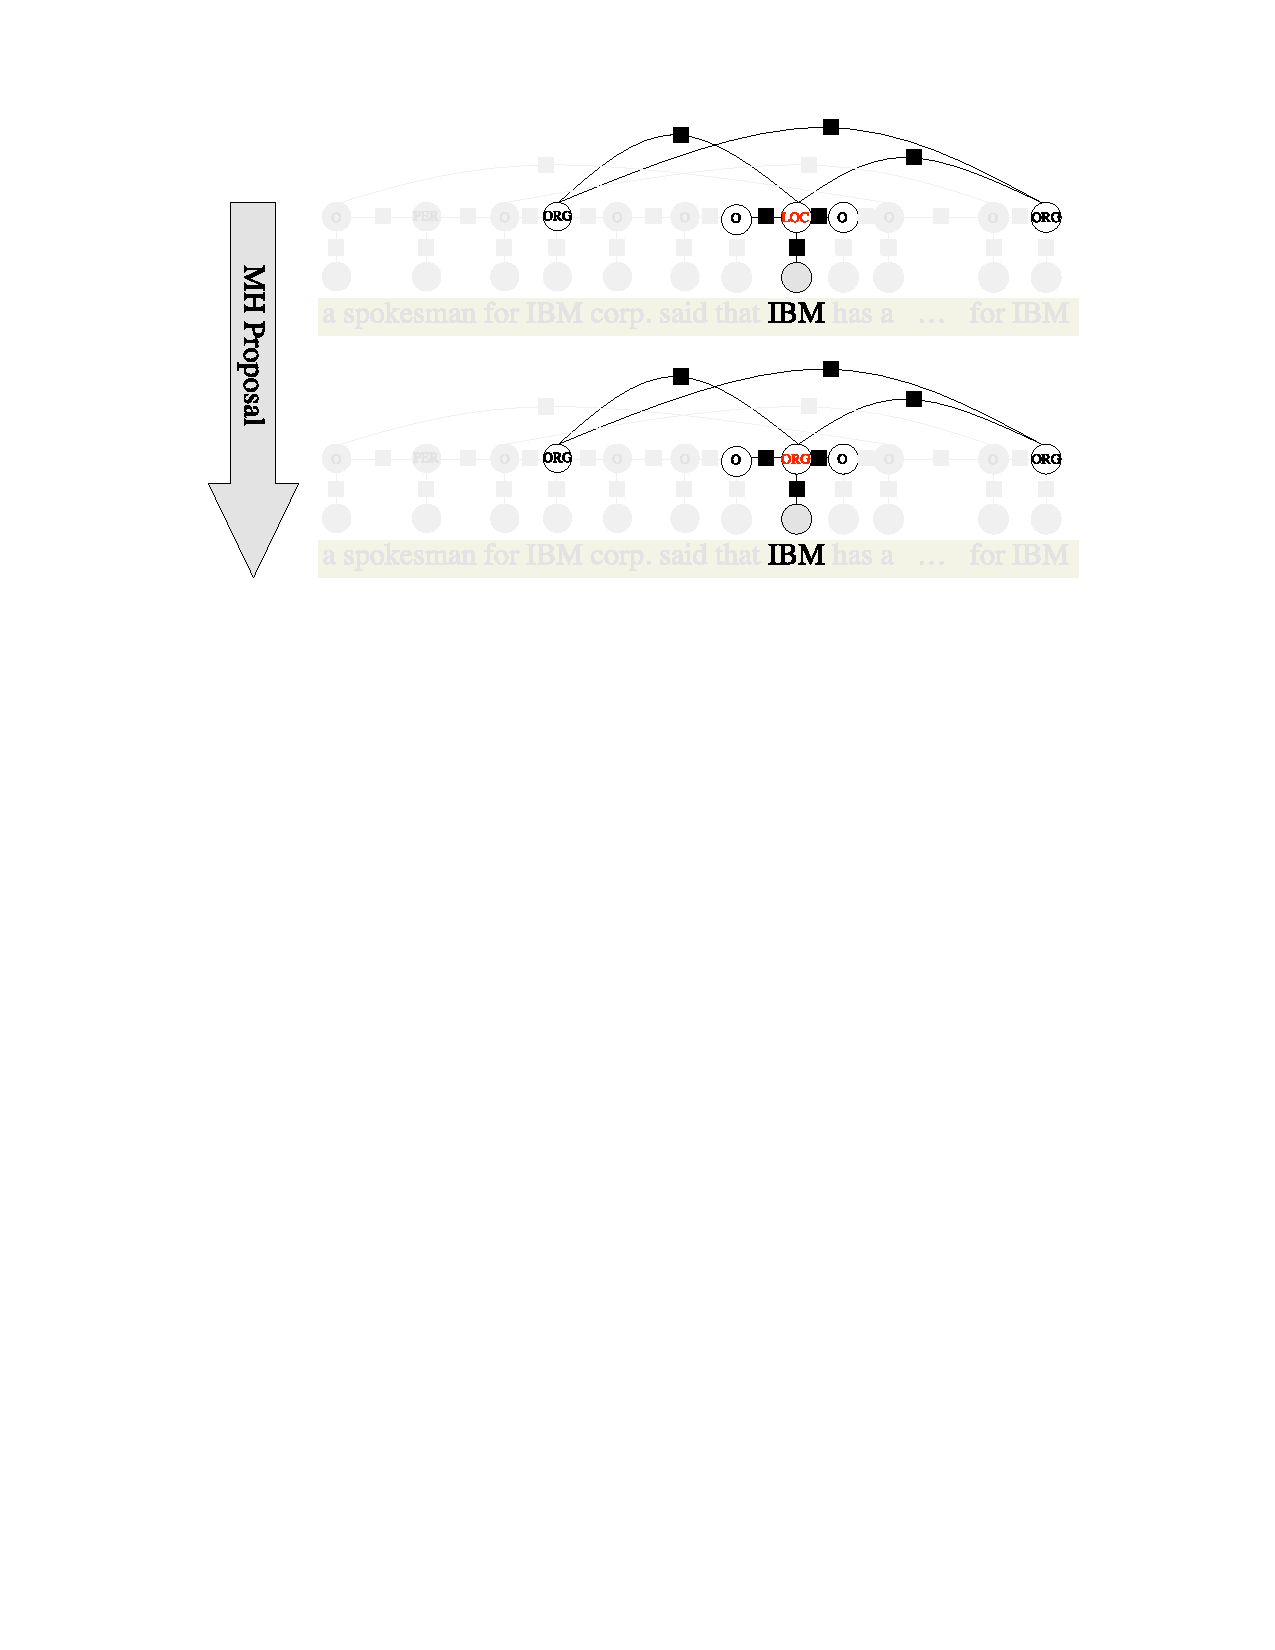
\includegraphics[width=.5\textwidth]{mcmc.pdf}
\end{figure}
Markov locality property allows for parallel computing.
\end{frame}


%% %---------- slide --------------------------------------------------%
%% \subsection{Inference Optimizer}
%% \begin{frame}{Inference Optimizer}
%% \begin{itemize}
%%   \item Incremental maintenance of MCMC samples.
%%   \item Parallel processing.
%%   \item Task decomposition and joint inference among subtasks.
%% \end{itemize}
%% \end{frame}


%% %---------- slide --------------------------------------------------%
%% \begin{frame}{Incremental Maintenance of MCMC Samples}
%% \head{Goal}
%% \begin{itemize}
%%   \item Evolve over time.
%%   \item Learn from past samples.
%%   \item Integrate new evidence.
%% \end{itemize}
%% \begin{figure}
%%   \centering
%%   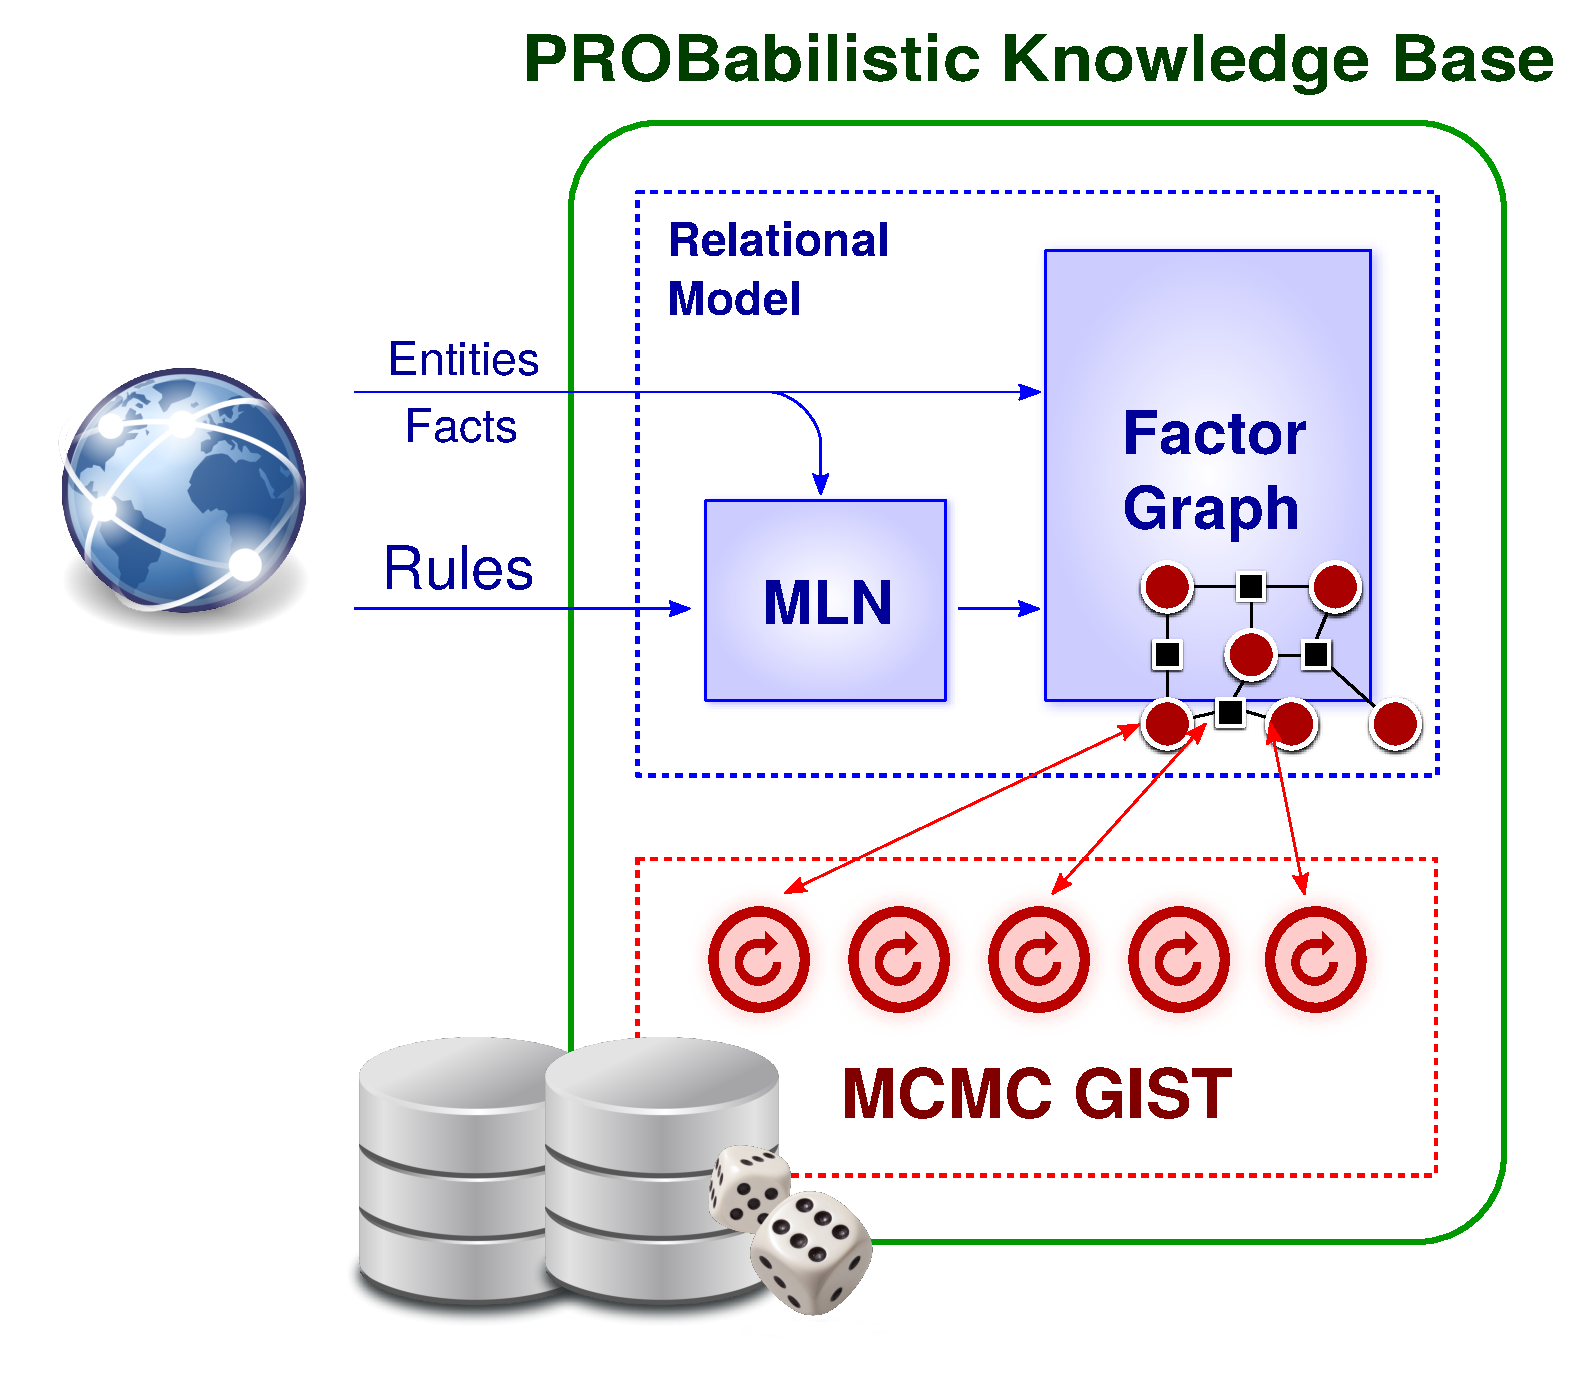
\includegraphics[clip,trim=50pt 350pt 50pt 30pt,width=.8\textwidth]{probkbarch.pdf}
%% \end{figure}
%% \end{frame}


%% %---------- slide --------------------------------------------------%
%% \begin{frame}{Incremental Maintenance of MCMC Samples}
%% \head{Query-Aware MCMC}
%% \begin{itemize}
%%   \item Focus computation on query nodes and nodes having more influence on query nodes.
%%   \item Proved to converge faster than traditional MCMC~\cite{DBLP:conf/nips/WickM11}. 
%% \end{itemize}

%% \head{Incremental MCMC}
%% The incremental maintenance algorithm adopts the same technique:
%% \begin{itemize}
%% \item Assumption: not much new information is added to the knowledge base each time.
%% \item Newly extracted knowledge serves as the query node.
%% \item Maintaining samples for both old and new nodes.
%% \end{itemize}
%% \end{frame}


%% %---------- slide --------------------------------------------------%
%% \begin{frame}{Incremental Maintenance of MCMC Samples}
%% The incremental MCMC proposal function $T$ employs the following steps:
%% \begin{enumerate}
%%   \item Sample the variable index space according to some distribution $p$ reflecting influence of new nodes and recent sample behaviors.
%%   \item Sample the selected variable according to some distribution $q$ over that variable's domain, leaving all other variables unchanged.
%% \end{enumerate}
%% We adjust the distribution $p$ so that it focuses on newly added variables.
%% \end{frame}


%% %---------- slide --------------------------------------------------%
%% \begin{frame}{MCMC Maintenance Results}
%% \begin{columns}[c]
%%   \column{0.46\textwidth}
%%   \begin{figure}
%%     \centering
%%     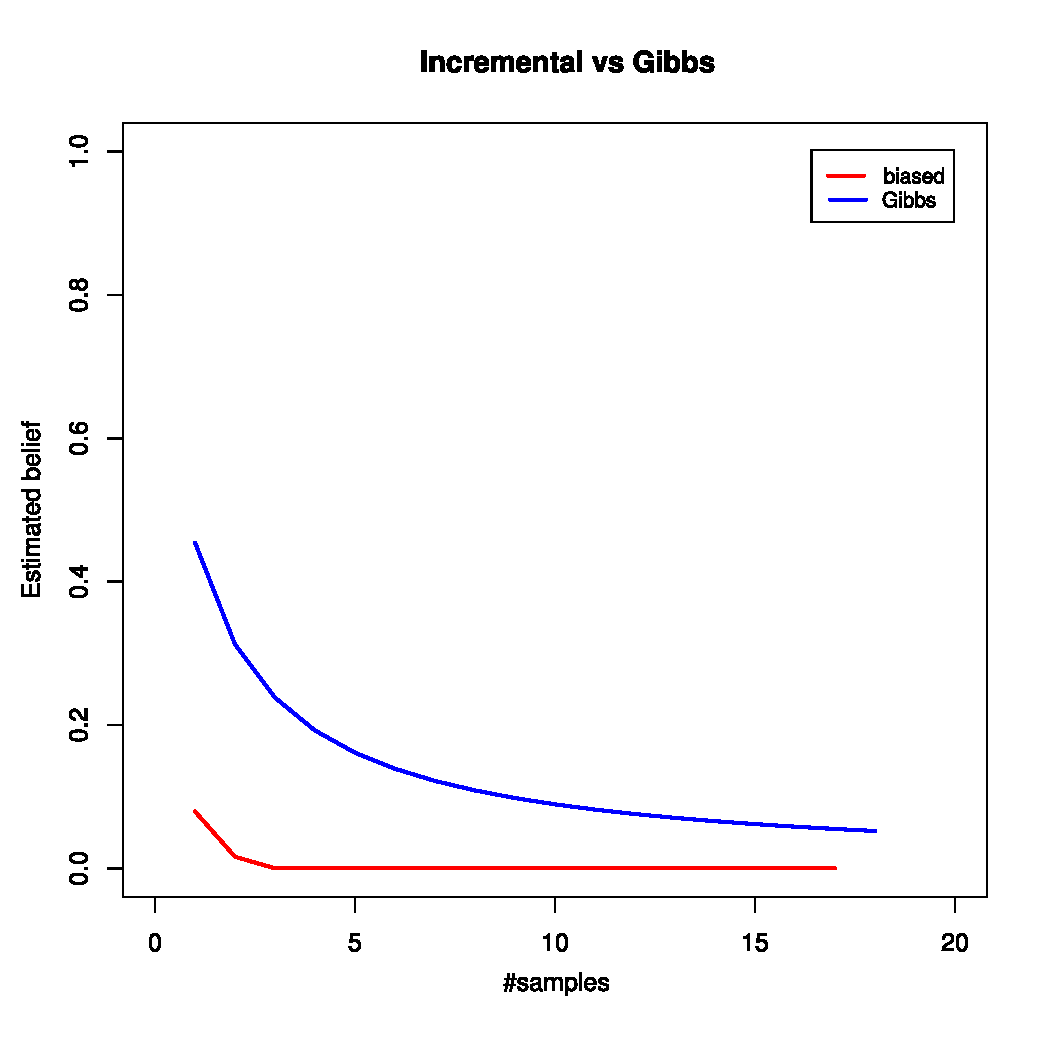
\includegraphics[width=\linewidth]{inc1.pdf}
%%   \end{figure}

%%   \column{0.46\textwidth}
%%   \begin{figure}
%%     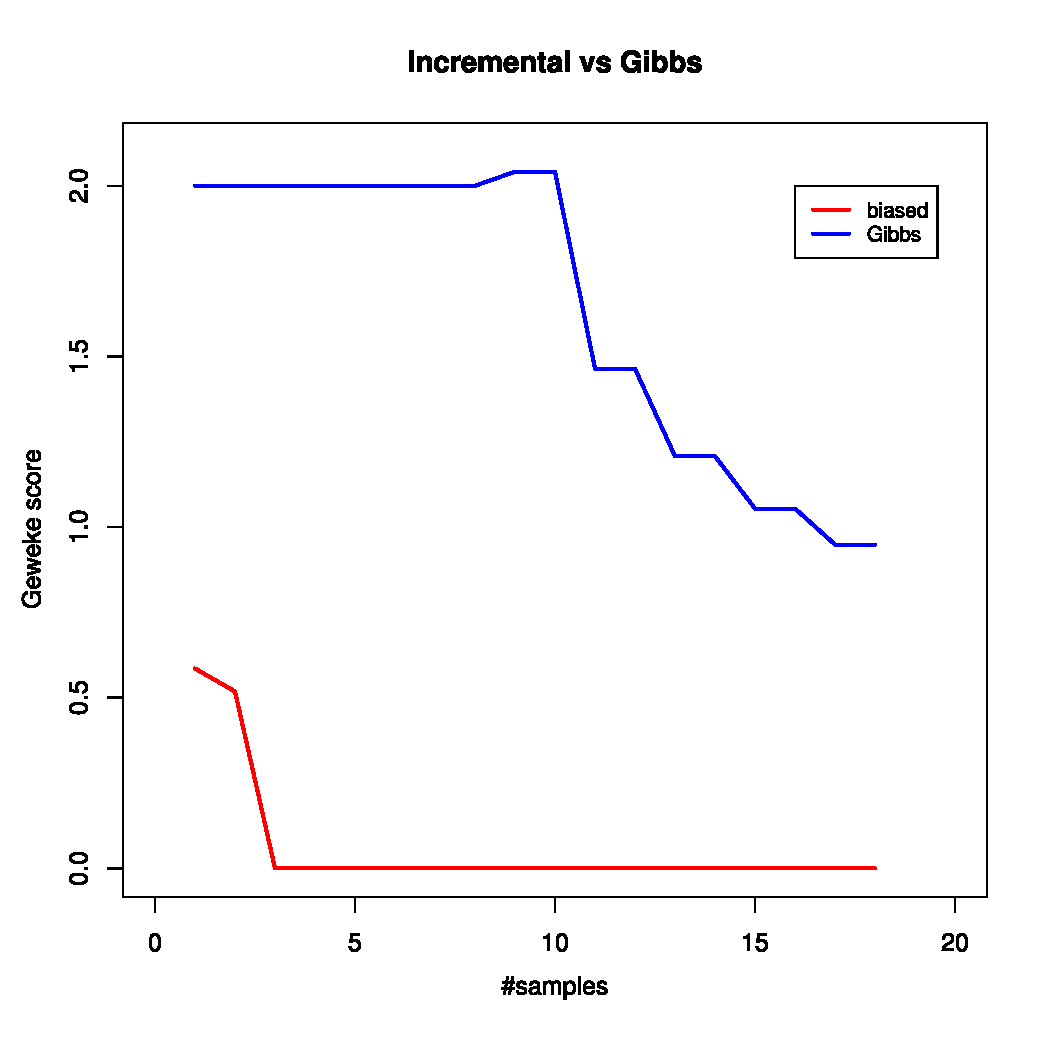
\includegraphics[width=\linewidth]{inc2.pdf}
%%   \end{figure}
%% \end{columns}

%% \textit{Note:} This algorithm is still under development.
%% \end{frame}


%---------- slide --------------------------------------------------%
\subsection{Parallel Processing Using GraphLab and Datapath}
\begin{frame}{GraphLab}
\begin{figure}
  \centering
  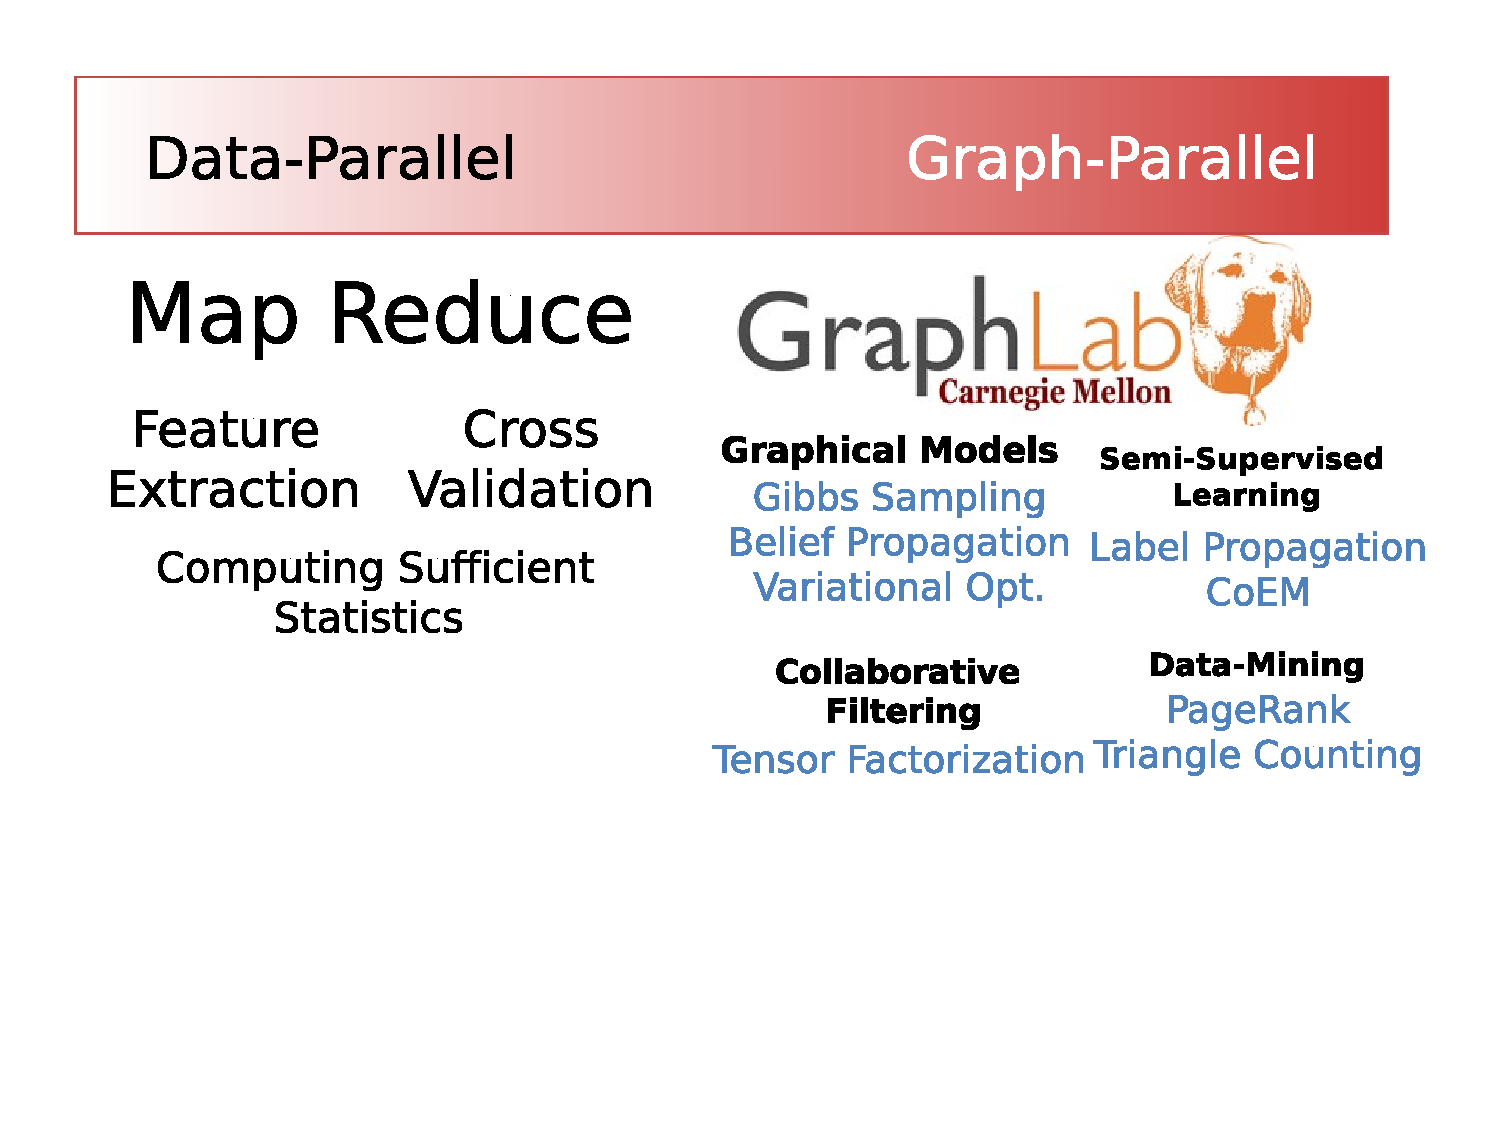
\includegraphics[clip,trim=20pt 150pt 20pt 30pt,width=.9\textwidth]{graphlab.pdf}
\end{figure}
\end{frame}


%---------- slide --------------------------------------------------%
%% \begin{frame}{GraphLab}
%% GraphLab~\cite{low2010graphlab,low2012distributed} is a framework for parallel machine learning that includes:
%% \begin{itemize}
%%   \item A graph-based data model representing data and computational dependencies.
%%   \item A set of consistency models.
%%   \item A sophisticated modular scheduling mechanism.
%%   \item Probabilistic graphical models inference algorithms.
%% \end{itemize}
%% \end{frame}

%---------- slide --------------------------------------------------%
\begin{frame}{GraphLab Execution Model}
\begin{algorithm}[H]\footnotesize
  \caption{\footnotesize GraphLab Execution Model}\label{alg:execution}
  \begin{algorithmic}
    \State\textbf{Input}: Data graph $G=(V,E,D)$
    \State\textbf{Input}: Initial vertex set $\mathcal{T}=\{v_1,v_2,\ldots\}$
    \While{$\mathcal{T}$ is not empty}
      \State $v\gets $\texttt{RemoveNext}($\mathcal{T}$)
      \State $(\mathcal{T}',\mathcal{S}_v)\gets f(v,\mathcal{S}_v)$
      \State $\mathcal{T}\gets\mathcal{T}\cup\mathcal{T}'$ 
    \EndWhile
    \State\textbf{Output}: Modified data graph $G=(V,E,D')$
  \end{algorithmic}
\end{algorithm}

\begin{itemize}
  \item Vertexes schedule execution of their neighbors.
  \item Not applicable to general MCMC algorithms.
\end{itemize}

\end{frame}

%---------- slide --------------------------------------------------%
\begin{frame}{Datapath \gist}
\head{Generalized Iterable State Transforms (GIST)}
\begin{itemize}
  \item GIST Performs \emph{transitions} upon a \emph{state} until that state has converged to the desired result.
  \begin{description}
    \item[Transition] MCMC Proposal function.
    \item[State] Factor graph with its samples.
  \end{description}
  \item A user-defined local scheduler allows general MCMC proposal implementation.
  \item The GIST state keeps track of the inference result.
\end{itemize}
\end{frame}

%---------- slide --------------------------------------------------%
%% \begin{frame}{Parallel Processing Using GraphLab}
%% We built a parallel-grounding, parallel-inference system on top of GraphLab.
%% \begin{figure}
%%   \centering
%%   \includegraphics[clip,trim=80pt 150pt 80pt 30pt,width=.75\textwidth]{distprobkb.pdf}
%% \end{figure}
%% \end{frame}


%---------- slide --------------------------------------------------%
\begin{frame}{GraphLab Preliminary Results}
\begin{table}
  \centering
  \rowcolors{1}{RoyalBlue!20}{RoyalBlue!5}
  \begin{tabular}{|cccccc|}\hline
    \textbf{\#samples} & 10 & 100 & 200 & 500 & State-of-the-art\\
    \hline
    \textbf{IE}   & 0.2s & 2s & 4s & 10.2s & 25.216s  \\
    \textbf{ER}   & 90.8s & 181.5s & 373s & $>$600s & 225s \\
    \textbf{RC}   & 5.2s & 52.7s & 111.3s & 297.8s & \textbf{\color{Red}Crashed} \\
    \sherlock-600 & 1.2s & 12.6s & 28.3s & 65.1s & 55min \\
    \hline
  \end{tabular}
  \caption{GraphLab-based parallel inference vs the state-of-the-art.}
\end{table}
\end{frame}

%---------- slide --------------------------------------------------%
\begin{frame}{Datapath Preliminary Results}
\begin{figure}
  \centering
  \caption{Inference over simulated factor graphs}
  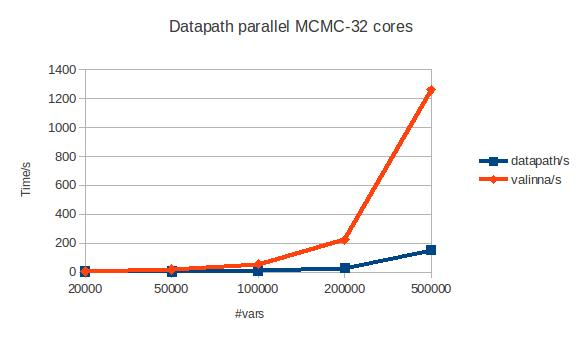
\includegraphics[width=.7\textwidth]{datapath.jpg}
\end{figure}
\end{frame}

%---------- slide --------------------------------------------------%
\subsection{Incremental MCMC (Future Work)}
\begin{frame}{Incremental MCMC (Future Work)}
A natural challenge arising in automatic knowledge-base construction is continuously incoming information.
\begin{itemize}
  \item Expanding frontier belief propagation (EFBP)~\cite{nath2010efficient} for repeated inference;
  \item Query-aware MCMC~\cite{wick2011queryaware} for query-spedific inference.
\end{itemize}
Following this line, we're trying to build an MCMC algorithm that:
\begin{itemize}
  \item Focuses computation on most recently added nodes.
  \item Maintains previous samples to avoid repeated computation.
\end{itemize}
\end{frame}

%---------- slide --------------------------------------------------%
\begin{frame}{Incremental MCMC (Future Work)}
\head{Challenges}
\begin{itemize}
  \item How to detect variables that are mostly affected by new ones.
  \item The biased nature of incremental MCMC poses inbalance to the Datapath scheduler.
\end{itemize}
\end{frame}


%% %---------- slide --------------------------------------------------%
%% \begin{frame}{Incremental MCMC}
%% \head{Goal}
%% \vspace{-6pt}
%% \begin{itemize}
%%   \item EFBP~\cite{nath2010efficient} in a MCMC setting
%% \end{itemize}

%% \head{Incremental MCMC}
%% The incremental maintenance algorithm adopts the Query-aware MCMC~\cite{wick2011queryaware} technique:
%% \begin{itemize}
%% \item Assumption: not much new information is added to the knowledge base each time.
%% \item Newly extracted knowledge serves as the query node.
%% \item Maintaining samples for both old and new nodes.
%% \end{itemize}
%% \end{frame}

%% %---------- slide --------------------------------------------------%
%% \begin{frame}{Incremental Maintenance of MCMC Samples}
%% The incremental MCMC proposal function $T$ employs the following steps:
%% \begin{enumerate}
%%   \item Sample the variable index space according to some distribution $p$ reflecting influence of new nodes and recent sample behaviors.
%%   \item Sample the selected variable according to some distribution $q$ over that variable's domain, leaving all other variables unchanged.
%% \end{enumerate}
%% We adjust the distribution $p$ so that it focuses on newly added variables.
%% \end{frame}

%---------- slide --------------------------------------------------%
%% \begin{frame}{MCMC Maintenance Results}
%% \begin{columns}[c]
%%   \column{0.46\textwidth}
%%   \begin{figure}
%%     \centering
%%     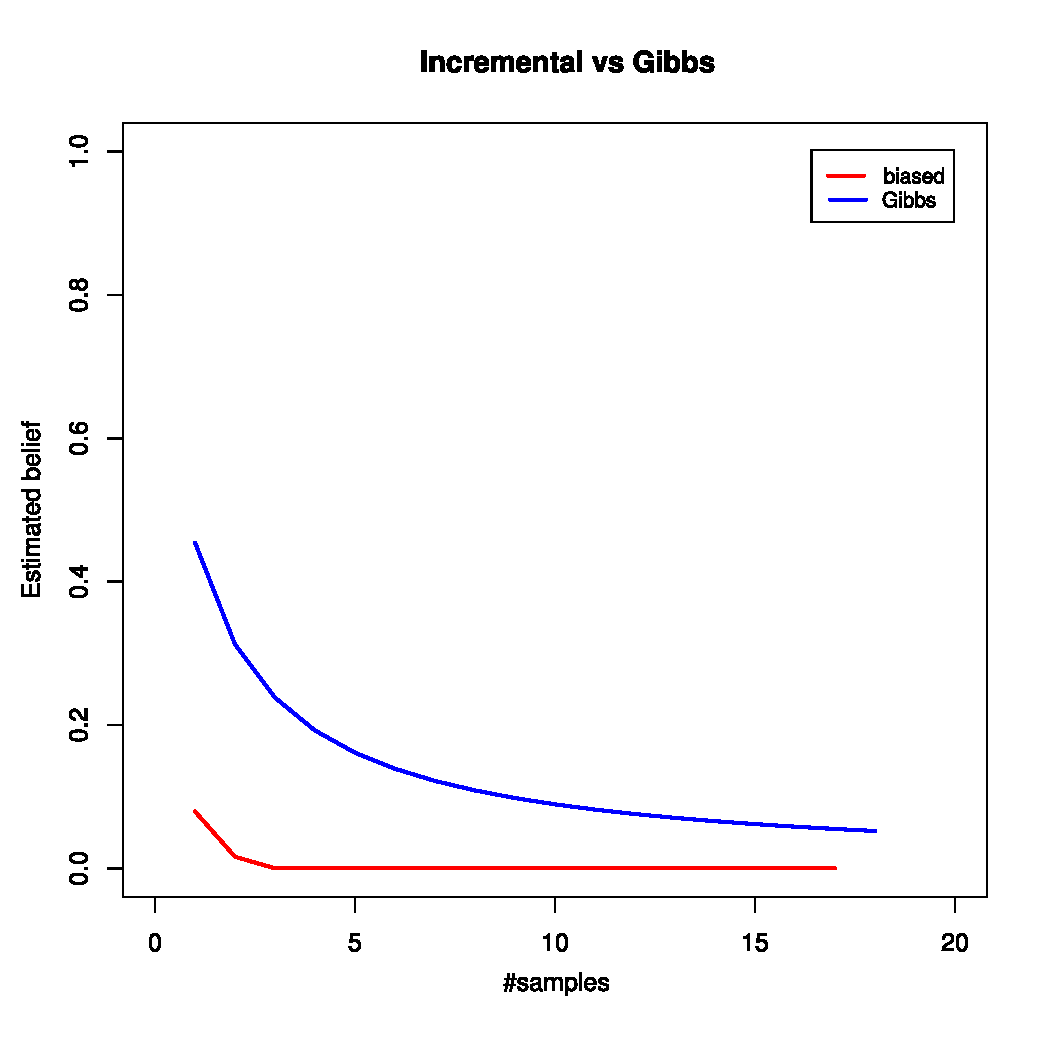
\includegraphics[width=\linewidth]{inc1.pdf}
%%   \end{figure}

%%   \column{0.46\textwidth}
%%   \begin{figure}
%%     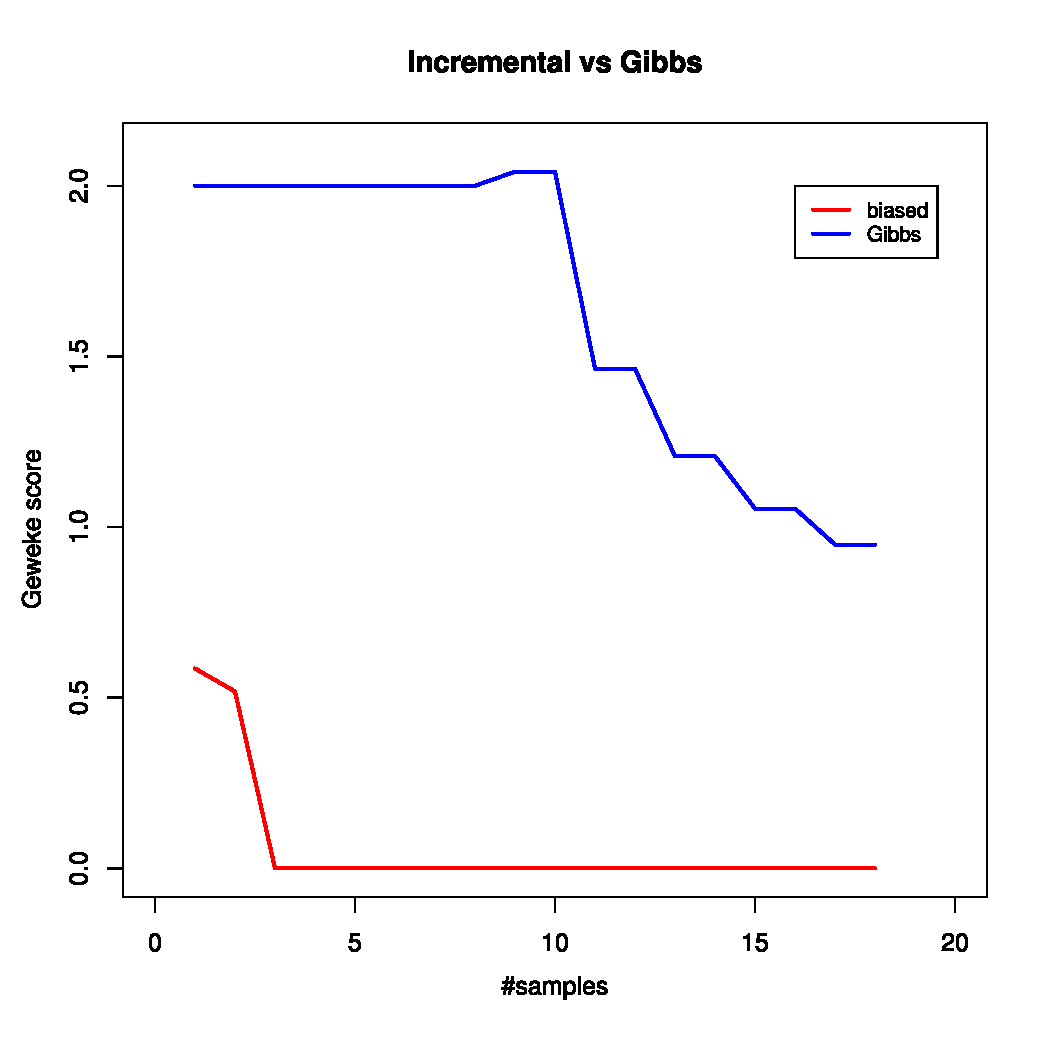
\includegraphics[width=\linewidth]{inc2.pdf}
%%   \end{figure}
%% \end{columns}

%% \textit{Note:} This algorithm is still under development.
%% \end{frame}

%% %---------- slide --------------------------------------------------%
%% \begin{frame}{Task Decomposition}
%% \felix~\cite{2011arXiv1108.0294N} proposes to decompose a generic MLN program into specialized tasks like CRF, classfication, coreference resolution, etc.
%% \begin{figure}
%%   \centering
%%   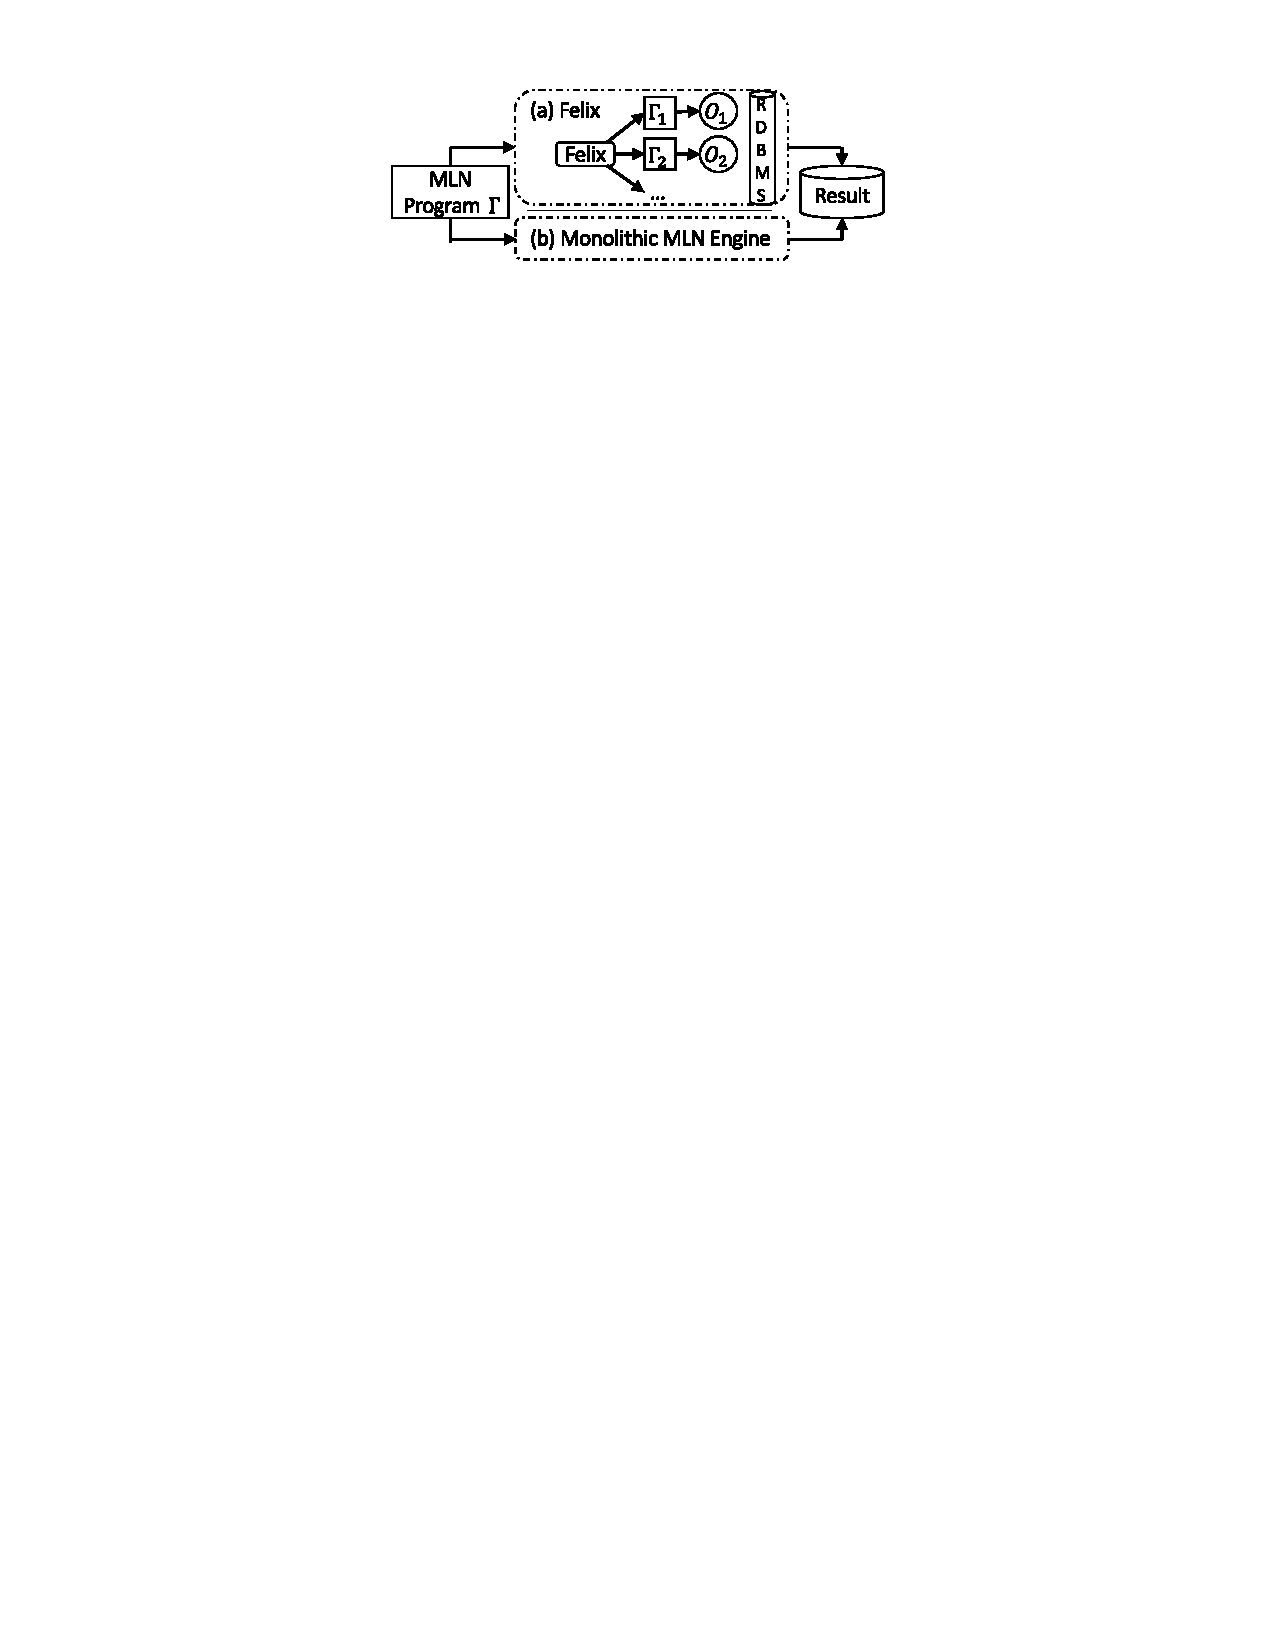
\includegraphics[clip,trim=170pt 665pt 170pt 40pt,width=.8\textwidth]{felix.pdf}
%% \end{figure}
%% \end{frame}


%% %---------- slide --------------------------------------------------%
%% \begin{frame}{Task Decomposition}
%% \head{Theoretical Foundation--Dual Decomposition}
%% Suppose we have an optimization problem
%% $$\min_{x_1,x_2,x_3} f(x_1,x_2,x_3)=f_1(x_1,x_2)+f_2(x_2,x_3).$$
%% It can be re-written as
%% $$\min_{x_1,x_{21},x_{22},x_3} f_1(x_1,x_{21})+f_2(x_{22},x_3)$$
%% $$\text{s.t. } x_{21}=x_{22}.$$
%% Introducing the Lagrangian multiplier $\lambda$, it becomes
%% $$\min_{x_1,x_{21},x_{22},x_3} f_1(x_1,x_{21})+f_2(x_{22},x_3)-\lambda(x_{21}-x_{22})$$
%% \end{frame}


%% %---------- slide --------------------------------------------------%
%% \begin{frame}{Task Decomposition}
%% \head{Theoretical Foundation--Dual Decomposition}
%% It is shown that we can instead solve the following optimization problem:
%% $$g(\lambda)=\min_{x_1,x_{21}}\left(f_1(x_1,x_{21})+\lambda x_{21}\right)+\min_{x_{22},x_3}\left(f_2(x_{22},x_3)-\lambda x_{22}\right).$$
%% To compute $\max_{\lambda}g(\lambda)$, we can use standard techniques such as projected subgradient~\cite{wolsey2000integer}.\\[5pt]

%% The decomposed problems can be solved more efficiently if we employ specialized algorithms for them.
%% \end{frame}


%% %---------- slide --------------------------------------------------%
%% \begin{frame}{Task Decomposition}
%% \begin{itemize}
%%   \item The \felix execution model works with text analysis applications where we wish to do joint inference between natural language processing and knowledge discovery.
%%   \item It does not work well with extracted rules since they don't fit the special rule patterns designed for \felix.
%%   \item Therefore, we propose to do \emph{two-level decomposition}:
%%   \begin{enumerate}
%%     \item template-level decomposition (the \felix model);
%%     \item instance-level decomposition (analyzing structures of graphical models).
%%   \end{enumerate}
%%   \item We haven't started this research but it is an exciting area to explore.
%% \end{itemize}
%% \end{frame}


%---------- slide --------------------------------------------------%
\begin{frame}{Conclusions}
\begin{itemize}
  \item \probkb is a web-scale \textbf{PROB}abilistic \textbf{K}nowledge \textbf{B}ase with Markov logic network as the primary data model.
  \item All extractions, including entities and rules, are stored in RDBMS as relational model, allowing efficient grounding algorithms.
  \item In-database \gist operator allows parallel MCMC inference.
  \item Incremental MCMC focuses computation on most recently added variables, speeding up convergence.
\end{itemize}
\end{frame}

%---------- slide --------------------------------------------------%
\begin{frame}{Questions?}
\begin{center}
  \LARGE Thank you!
\end{center}
\end{frame}


%---------- slide --------------------------------------------------%
\section{References}
\subsection{References}
\begin{frame}[allowframebreaks]{References}
  \bibliographystyle{alpha}
  \bibliography{probkb}
\end{frame}

\end{document}
